\documentclass[final_report_innit.tex]{subfiles}

\begin{document}

\section{Survey Results Analysis}

In this section, we will present our survey results, on the basis of which we hope to identify the applicability of process and design activities to the manual coding and MDSD paradigms. Our survey questions have provided us with data on five process and design activities: continuous integration (CI), cross-functional teams (CFT), One Track (OT), unit testing (UT) and component testing (CT). We have measured the impact of these activities with regard to performance and productivity, quality of deliverables, personal fulfillment and ease of implementation.
\\

The survey data came from twenty questionnaires which were sent to employees at Ericsson, specifically those working in the EPG department. Our contact at Ericsson distributed them between the manual coding and MDSD practitioners. We received fourteen replies, and out of those six were from the MDSD practitioners and eight from manual coding. Out of those responses we deemed that four responses from the MDSD practitioners were suitable and that seven from the manual coding practitioners were also suitable. Suitability was derived from how complete the answer sets were, for example, most of the responses which were stricken were missing well over 50\% of the answers and thus were unsuited for analysis.
\\

When analysing the data we decided not to perform any complicated statistical analysis. The primary motivation for this was the scale of the data set that we had collected; had we collected more, a more extensive statistical analysis would have been appropriate. To generate our averages, we simply calculated the mean responses by grouping the answers according the process and design activities. We generated an average for each of MDSD and manual coding in relation to the design and process questions. We then generated an average of all the questions and finally generated averages from each question block for MDSD and manual coding, ending with an average of both of these together. The final part of the analysis involved an interview with our contact at Ericsson. The interview provided additional insight into some of the design and process elements which they utilise, especially those that we were particularly interested in.
\\

With regard to CFT, the interviewee seemed to be in agreement with the positive responses of both manual coding and MDSD practitioners, since the interviewee indicated that their change is completed and part of the culture at EPG. However, considering the discrepancy of responses on CI, the interviewee expressed that the discontent of manual coding practitioners was unexpected, since the interviewee believed that CI should be as applicable to the manual coding paradigm as to the MDSD paradigm. Overall, the interview that we conducted with our contact at EPG helped us to formulate our assumptions about the survey results. 
\\
\\

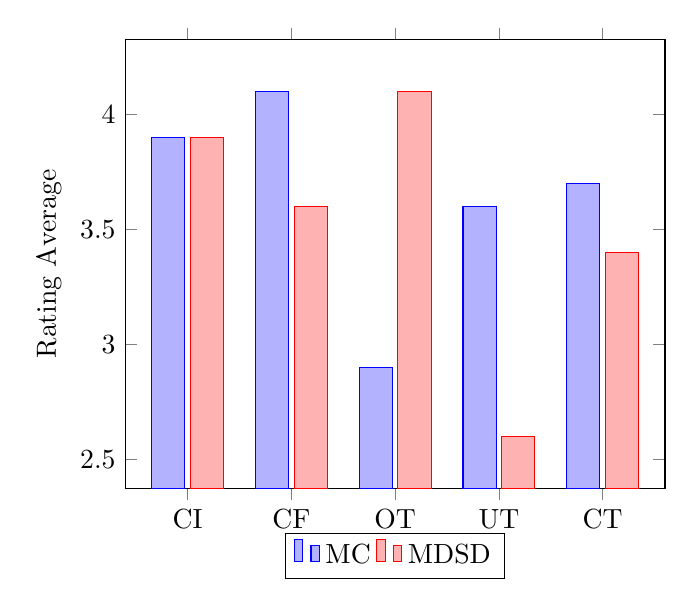
\begin{tikzpicture}
\begin{axis}[
	every axis plot post/.style={/pgf/number format/fixed},
	symbolic x coords={CI, CF, OT, UT, CT},
	ylabel=Rating Average,
	enlargelimits=0.15,
	legend style={at={(0.5,-0.1)},
	anchor=north,legend columns=-1},
	%ybar interval=0.7,
	ybar,
	bar width=12pt
]
\addplot 
	coordinates {(CI,3.9) (CF,4.1)
		 (OT,2.9) (UT,3.6) (CT,3.7)};
\addplot 
	coordinates {(CI,3.9) (CF,3.6) 
		(OT,4.1) (UT,2.6) (CT,3.4)};
\legend{MC,MDSD}
\end{axis}
\end{tikzpicture}

\begin{center}\textit{Response Average of manual coding and MDSD respondents for Process and Design Activities}\end{center}

\begin{table}[h]
\caption{Process Activity Survey Results}
\centering
\begin{tabular}{@{}l|c|c|c|@{}}
\cmidrule(l){2-4}
                             & \multicolumn{1}{l|}{avg(MC)} & \multicolumn{1}{l|}{avg(MDSD)} & \multicolumn{1}{l|}{avg(all)} \\ \midrule
\multicolumn{1}{|l|}{CI-P}   & 4.1                          & 4.0                           & 4.1                           \\ \midrule
\multicolumn{1}{|l|}{CI-Q}   & 3.6                          & 4.0                           & 3.7                           \\ \midrule
\multicolumn{1}{|l|}{CI-PF}  & 3.4                          & 3.0                           & 3.3                           \\ \midrule
\multicolumn{1}{|l|}{CI-EOI} & 4.3                          & 4.5                           & 4.4                           \\ \midrule
\multicolumn{1}{|l|}{CF-P}   & 4.3                          & 4.0                           & 4.3                           \\ \midrule
\multicolumn{1}{|l|}{CF-Q}   & 4.0                          & 1.0                           & 3.6                           \\ \midrule
\multicolumn{1}{|l|}{CF-PF}  & 3.7                          & 3.0                           & 3.5                           \\ \midrule
\multicolumn{1}{|l|}{CF-EOI} & 4.5                          & 5.0                           & 4.6                           \\ \midrule
\multicolumn{1}{|l|}{OT-P}   & 3.2                          & 4.0                           & 3.6                           \\ \midrule
\multicolumn{1}{|l|}{OT-Q}   & 3.2                          & 4.5                           & 3.8                           \\ \midrule
\multicolumn{1}{|l|}{OT-PF}  & 3.0                          & 3.0                           & 3.0                           \\ \midrule
\multicolumn{1}{|l|}{OT-EOI} & 2.2                          & 4.5                           & 3.2                           \\ \bottomrule
\end{tabular}
\end{table}

\begin{table}[h]
\caption{Design Activity Survey Results}
\centering
\begin{tabular}{@{}l|c|c|c|@{}}
\cmidrule(l){2-4}
                             & \multicolumn{1}{l|}{avg(MC)} & \multicolumn{1}{l|}{avg(MDSD)} & \multicolumn{1}{l|}{avg(all)} \\ \midrule
\multicolumn{1}{|l|}{UT-P}   & 3.5                          & 3.0                           & 3.4                           \\ \midrule
\multicolumn{1}{|l|}{UT-Q}   & 4.0                          & 3.0                           & 3.8                           \\ \midrule
\multicolumn{1}{|l|}{UT-PF}  & 3.3                          & 3.0                           & 3.3                           \\ \midrule
\multicolumn{1}{|l|}{UT-EOI} & 3.5                          & 1.7                           & 2.9                           \\ \midrule
\multicolumn{1}{|l|}{CT-P}   & 3.7                          & 4.0                           & 3.8                           \\ \midrule
\multicolumn{1}{|l|}{CT-Q}   & 4.7                          & 5.0                           & 4.8                           \\ \midrule
\multicolumn{1}{|l|}{CT-PF}  & 3.0                          & 3.0                           & 3.0                           \\ \midrule
\multicolumn{1}{|l|}{CT-EOI} & 3.3                          & 2.5                           & 2.9                           \\ \bottomrule
\end{tabular}
\end{table}

\begin{table}[h]
\caption{Design and Process Activity Averages}
\centering
\begin{tabular}{@{}c|c|c|c|@{}}
\cmidrule(l){2-4}
\multicolumn{1}{l|}{}    & \multicolumn{1}{l|}{avg/activity(MC)} & \multicolumn{1}{l|}{avg/activity(MDSD)} & \multicolumn{1}{l|}{avg/activity(all)} \\ \midrule
\multicolumn{1}{|c|}{CI} & 3.9                                & 3.9                                 & 3.9                                 \\ \midrule
\multicolumn{1}{|c|}{CF} & 4.1                                & 3.6                                 & 4.0                                 \\ \midrule
\multicolumn{1}{|c|}{OT} & 2.9                                & 4.1                                 & 3.4                                 \\ \midrule
\multicolumn{1}{|c|}{UT} & 3.6                                & 2.6                                 & 3.3                                 \\ \midrule
\multicolumn{1}{|c|}{CT} & 3.7                                & 3.4                                 & 3.5                                 \\ \bottomrule
\end{tabular}
\end{table}

\noindent
\textit{
\textbf{\hspace{12 mm}Table legend:}
\\
\hspace*{13 mm}P - Performance
\\
\hspace*{13 mm}Q - Quality
\\
\hspace*{13 mm}PF - Personal Fulfilment
\\
\hspace*{13 mm}EOI - Ease of Implementation
}

\end{document}